\documentclass[10pt,twocolumn]{article}
\usepackage{times}
\usepackage{multirow}
\usepackage{graphicx,grffile}
\usepackage{pgf}
\usepackage{tikz}
\usetikzlibrary{arrows,automata}
\usepackage[latin1]{inputenc}

% do not change these values
\baselineskip 12pt
\textheight 9in
\textwidth 6.5in
\oddsidemargin 0in
\topmargin 0in
\headheight 0in
\headsep 0in

%\makeatletter
%\def\maxwidth{\ifdim\Gin@nat@width>\linewidth\linewidth\else\Gin@nat@width\fi}
%\def\maxheight{\ifdim\Gin@nat@height>\textheight\textheight\else\Gin@nat@height\fi}
%\makeatother
%% Scale images if necessary, so that they will not overflow the page
%% margins by default, and it is still possible to overwrite the defaults
%% using explicit options in \includegraphics[width, height, ...]{}
%\setkeys{Gin}{width=\maxwidth,height=\maxheight,keepaspectratio}
%

\usepackage[unicode=true]{hyperref}
\hypersetup{breaklinks=true,
            bookmarks=true,
            pdfauthor={},
            pdftitle={},
            colorlinks=true,
            citecolor=blue,
            urlcolor=blue,
            linkcolor=blue,
            pdfborder={0 0 0}}
\urlstyle{same}  % don't use monospace font for urls

\usepackage[font=footnotesize,labelfont=bf]{caption}

\begin{document}

\title{title}

\author{
%Noah Watkins, Neha Ojha\textsuperscript{*}, Carlos Maltzahn \\
%\small {\em University of California, Santa Cruz} \\
%\small {\{jayhawk,carlosm\}@cs.ucsc.edu} \textsuperscript{*}nojha@ucsc.edu \\ [2mm]
\small Submission Type: Research
}

\date{}
\maketitle

\begin{abstract}
abstract
\end{abstract}

\section{Introduction}

Cloud providers are increasingly reliant upon application-specific extensions
to distributed storage system such as Ceph as is shown in
Figure~\ref{fig:objclass-dev} by a marked increase in Ceph extensions used in
production.

The construction of extensions is not limited to core developers; the
development community has been receptive to contributions with the recent
inclusion by CERN developers of an extension for performing limited numeric
operations on object data~\cite{cls_numops}.

This trend is not limited to Ceph. AWS Lambda, Redis Lua, Redis Modules,
KV-Drives, and Rhea, are all recent examples of storage systems embracing the
power of including application-specific semantics. While Ceph has not yet
reached the point of directly exposing these features to users, the recent
inclusion of a mechanism for dynamically defining extensions using
Lua~\cite{cls_lua} suggests that aspects of this may soon appear.

If the growth illustrated in Figure~\ref{fig:objclass-dev} continues, the
amount of low-level C++ is likely to grow very larage. Unfortunately, much of
this code is written assuming a performance profile defined by a combination
of the hardware and software versions available at the time of development. As
Ceph development continues at a fast pace, the cost of adapting to changing
assumptions regarding performance will become significant.

% footnote: we could probably look through the cls_* changelog and find
% examples of changes based on changes to semantics.

% Virtualization. Operating systems and containers are similar. AUFS, dockerfile

In order to avoid this we need declarative magic hats.

\section{Recurring Problem}


Describe CORFU briefly, and then show the physical design challenge. The
performance decision changes depending on the mix of hardware and software
versions and configurations.





\section{Storage System Programmability}

\begin{figure}[ht]
  \centering
    \includegraphics[width=0.45\textwidth]{experiments/objclass-dev/output.png}
    \caption{
[\href{https://github.com/noahdesu/zlog-popper/tree/master/experiments/objclass-dev/visualize.ipynb}{source}]
Growth of officially supported, custom object interfaces in RADOS over 6
years. A \emph{method} is a specific object interface and a \emph{class} is a
logical grouping of methods.
}
\label{fig:objclass-dev}
\end{figure}

When application goals are not met by a storage system the most common reaction
is to design a workaround. Workarounds roughly fall into one of two categories:
so called ``bolt-on'' services that introduce a 3rd party system (e.g. a
metadata service), or expanded application responsibility in the form of data
management (e.g. a new data layout).

\section{Consolidated Section}

Up until this point we have introduced Ceph, CORFU, the general problems
associated with programmability, described ZLog as being an instantiation of
the CORFU interface on top of Ceph.

Template for the CORFU object class interface. Maybe a simple state machine.

Describe indexing and protocol enforcement.
Differences between built-in interfaces and custom cls interfaces.


\section{ZLog Physical Design}

In this section we examine the design space for implementing the CORFU
protocol in the RADOS storage system. Table \ref{t:init-ds} shows the entire
design space. A description of each design parameter follows:

{\bf Mapping strategy.} The method by which a log entry---identified by its
logical position---is addressed within RADOS is referred to as the mapping
strategy. A 1:1 strategy stores each log entry in a RADOS object with a
distinct name (e.g. ``mylog.pos443''), and an N:1 strategy stripes the log
positions across a set of objects (e.g.  round-robin). While we do consider
both strategies in this paper, a 1:1 strategy is attractive because it allows
a design in which clients can directly address log positions by constructing
the correct object name.

{\bf Storage interface.} entry data may be small or large. its primary
storage location is important. kv, bs. we further sub-divide bs into
write and append. each strategy is compatible with fixed size entries
except for the write interface.

{\bf Logical addressing.}

\subsection{Storage Interface Selection}

Figure \ref{f:librados-sweep} shows the single-node write-only I/O throughput
for each of the points in the design space defined in Table \ref{t:init-ds}.
The results reveal poor relative performance using both the key-value storage
interface, as well as either of the 1:1 strategies---which incur overhead by
creating a new object for each log entry. Both of the N:1 strategies using the
bytestream I/O interface outperform all of the other approaches by over 2x
throughput, but otherwise have nearly identical performance.

To examine the read performance of the points in the design space we generated
a dataset using each of the write workloads, and then issued random reads
across the entire dataset. Figure \ref{f:librados-rand-read} shows the read
throughput for each of the design strategies. The results show that an N:1
mapping using bytestream interface performs best. Interestingly, the 1:1
mapping strategy using the bytestream interface exhibits good read performance
in comparison to writes using the same strategy.

\begin{table}
\begin{tabular}{|l|l|l|}
\hline
Category & Specialization & Methods \\ \hline
\multirow{2}{*}{Locking} & Shared & \multirow{2}{*}{6} \\
                         & Exclusive & \\ \hline
\multirow{3}{*}{Logging} & Replica & 3 \\
                         & State & 4 \\
                         & Timestamped & 4 \\ \hline
Garbage Collection & Reference Counting & 4 \\ \hline
\multirow{4}{*}{Metadata Management} & RBD & 37 \\
 & RGW & 27 \\
 & User & 5 \\
 & Version & 5 \\ \hline
\end{tabular}
\caption{A variety of RADOS object storage classes exist that expose reusable interfaces to applications.}
\label{tab:objclasses}
\end{table}


\begin{figure}
\centering
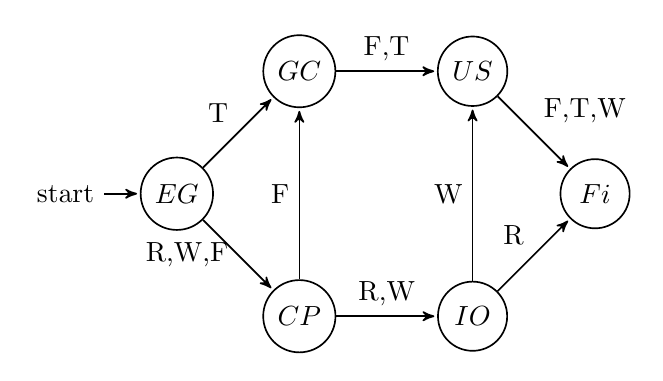
\begin{tikzpicture}[->,>=stealth',shorten >=1pt,auto,node distance=2.2cm,semithick]
%\tikzstyle{every state}=[fill=red,draw=none,text=white]

  \node[initial left,state] (A)              {$EG$};
  \node[state]         (B) [below right of=A] {$CP$};
  \node[state]         (D) [right of=B]       {$IO$};
  \node[state]         (C) [above right of=A] {$GC$};
  \node[state]         (E) [right of=C]       {$US$};
  \node[state]         (F) [below right of=E] {$Fi$};

  \path (A) edge        node [left] {R,W,F} (B)
            edge        node {T}     (C)
        (B) edge        node {F}     (C)
            edge        node {R,W}   (D)
        (C) edge        node {F,T}   (E)
        (D) edge        node {W}     (E)
            edge        node {R}     (F)
        (E) edge        node {F,T,W} (F);
\end{tikzpicture}
\caption{State transition diagram for read ($R$), write ($W$), fill ($F$), and
trim ($T$) CORFU operaitons. The states epoch guard ($EG$), check position ($CP$),
and update state ($US$) access metadata. The I/O performs a log entry read or
write, and garbage collection ($GC$) marks entries for reclamation.}
\end{figure}


\begin{table}
\begin{tabular}{ | l | l | l | l | l |}
\hline
Map & I/O & Entry Size & Addressing & Metadata \\ \hline
\multirow{2}{*}{1:1} & KV  & Flex     & Ceph      & KV/BS \\ \cline{2-5}
                     & BS  & Flex     & Ceph/VFS  & KV/BS \\ \hline
\multirow{4}{*}{N:1} & KV  & Flex     & \multicolumn{2}{|c|}{KV/BS} \\ \cline{2-5}
                     & WR  & Fixed    & VFS       & KV/BS \\ \cline{2-5}
                     & AP  & Flex     & KV/BS     & KV/BS \\
\hline
\end{tabular}
\caption{The high-level design space of mapping CORFU log entry storage onto
the RADOS object storage system.}
\label{t:init-ds}
\end{table}

\begin{figure}[h]
  \centering
  \includegraphics[width=0.45\textwidth]{experiments/librados-sweep/output.soft.reset.2hr.png}
  \caption{
[\href{https://github.com/noahdesu/zlog-popper/tree/master/experiments/librados-sweep/visualize.ipynb}{source}]
Throughput (IOPS) of 1K writes to a single OSD using the standard I/O
interfaces in various configurations. The best performance is achieved using
the byte stream interface and a N:1 mapping strategy.
}
\end{figure}

\begin{figure}[h]
  \centering
  \includegraphics[width=0.45\textwidth]{experiments/basic-cls-rand-read/output.read.60min.png}
  \caption{
[\href{https://github.com/noahdesu/zlog-popper/tree/master/experiments/basic-cls-rand-read/visualize.ipynb}{source}]
Throughput of 1K random reads to a single OSD using the standard I/O
interfaces in various configurations. The best performance is achieved using
the byte stream interface and a N:1 mapping strategy.
}
\end{figure}

As a first approximation these results show that when optimizing for log
append and random read throughput the design space should be refined by
limiting solutions to architectures based on a N:1 mapping strategy using the
bytestream I/O interface. But what these microbenchmarks explicitly omit are
the overheads associated with metadata management such as enforcing write-once
semantics or using an index to map a log position to a physical offset within
an object. In the next section we

\subsection{Metadata Management}

\begin{figure}[h]
  \centering
  \includegraphics[width=0.45\textwidth]{experiments/basic-cls-overhead/output.1024.soft.reset.png}
  \caption{
[\href{https://github.com/noahdesu/zlog-popper/tree/master/experiments/basic-cls-overhead/visualize.ipynb}{source}]
}
\end{figure}

Many variations of design here. What is the easiest way to 
winnow down the design space.

NEXT GRAPH A

This is an easy interface to simulate.
- Check Epoch (omap, stream header)
- this graph also has the APPEND raw through for comparison
- adds NEW OSD OP TO AVOID CLS OVERHEAD DISCUSSION FOR PAPER
- 3 runs in this graph, no need to write interface
- short runs to verify and then do all long runs togther with next graph

Both protocol enforcement and logical address translation
represent a larger design space involving index design. However
since in either case all state must be stored in the omap and
in the stream header, testing the overhead of epoch enforcement
provides a strict upper bound on performance.

- Protocol Enforcement
- Logical Translation (only append case)

Memory Cache

NEXT GRAPH B (or combined with A)
Use in-memory cache to implement the epoch check and show that we can match
the raw performance even with this added functionality.
This will show the content from graph A for comparison. Look
we match the raw performance.

NEXT GRAPH B or C (probably just two).. bar chart?
 Final consolidation of average throughputs of all the different
methods
 THIS INCLUDES THE FULL IMPL OF ZLOG APPEND using the in-memory cache

We solve the slow down of the epoch by storing the value in memory. Here is
the new performance.  We are able to with the epoch check match the raw
performance.

We know that we cannot use kv/bs for logicla address translation or protocol
enforcement without a performance hit so there is no point in trying. instead,
we generalize this memory cache hting used for epoch checks as a
new interface and use this interface to implement the full zlog
stack and show the performance.

Overall corfu is relatively simple abtraction, yet requires significant
work in making performant. Further, the decision may change over time.

We will probably have room in the paper to discuss the design of the
index structure, like collapsing a bit map and taking advantage of
the implicit strides in the offsets, etc... but we can probably move
that to a later section to keep this presentation concise. We should
probably mention this aspect here, but overall that becomes a ortholognal
optimization.

%# Abstract Model

%# Sequencer Creation

\bibliography{paper}
\bibliographystyle{plain}

\end{document}
